\begin{frame}
\huge
\centering
    Introducción
\end{frame}
%----------

\subsection{Global}% Referencia FSB sobre mayor interconexión con el sector financiero tradicional

\begin{frame}
\frametitle{Incremento en las \textcolor{cyan}{interconexiones} con los mercados financieros tradicionales. FSB 2022.}

        \begin{figure}[H]
        \begin{center}
         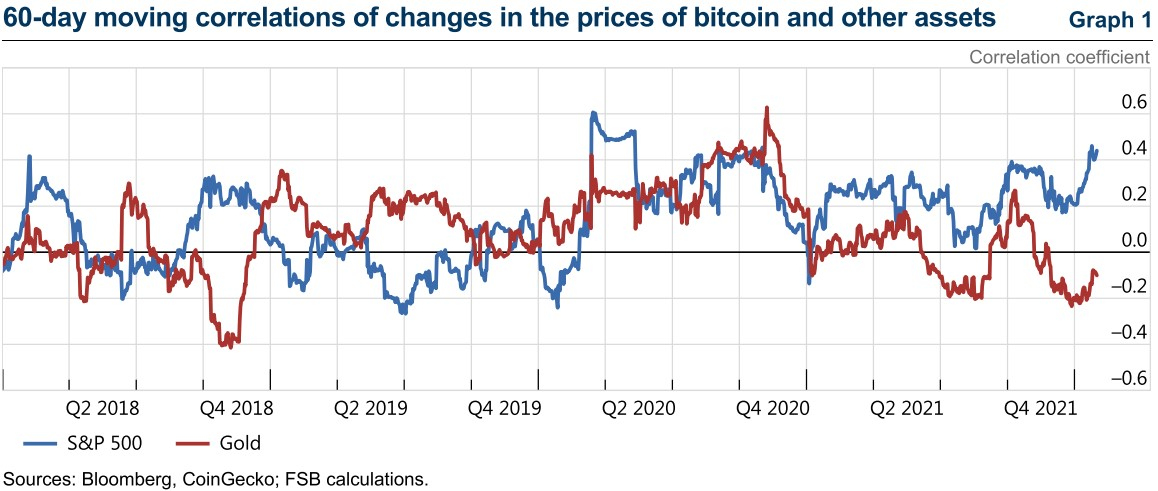
\includegraphics[width=1\textwidth]{images/C1/FSB 2022 correlation.jpg}
         \end{center}
        \end{figure}
\note{
\begin{itemize}
\item El FSB llega a esta conclusión luego de analizar:
    \begin{itemize} 
    \item El nivel de capitalización de mercado de los criptoactivos, la cual creció 3.5 veces en 2021 hasta 2.6 billones (a inicios de marzo se encuentra próxima a los dos billones).
    \item El rápido crecimiento de las conexiones directas entre los criptoactivos y las instituciones financieras de importancia sistémica y los mercados financieros centrales (si bien de niveles bajos).
    \item El incremento durante 2021 de la participación institucional en los mercados de criptoactivos, tanto como inversores como proveedores de servicios.
    \item El incremento en el nivel de conexiones entre criptoactivos e instituciones financieras sistémicas puede asociarse al incremento en la correlación entre la variación en el precio de bitcoin y otros activos tradicionales. 
    \item Cómo se observa en el gráfico, la correlación entre las variaciones en el precio de bitcoin y las variaciones en el índice SP500 ha tendido a incrementarse. De hecho, según la consultora Coinmetrics, el coeficiente se encuentra próximo a o.5 para estos primeros meses del 2022. 
    \end{itemize}
\end{itemize}
}
\end{frame}
%----------

\subsection{Local}

\begin{frame}
\frametitle{Operaciones p2p}

    \begin{figure}
    \centering
        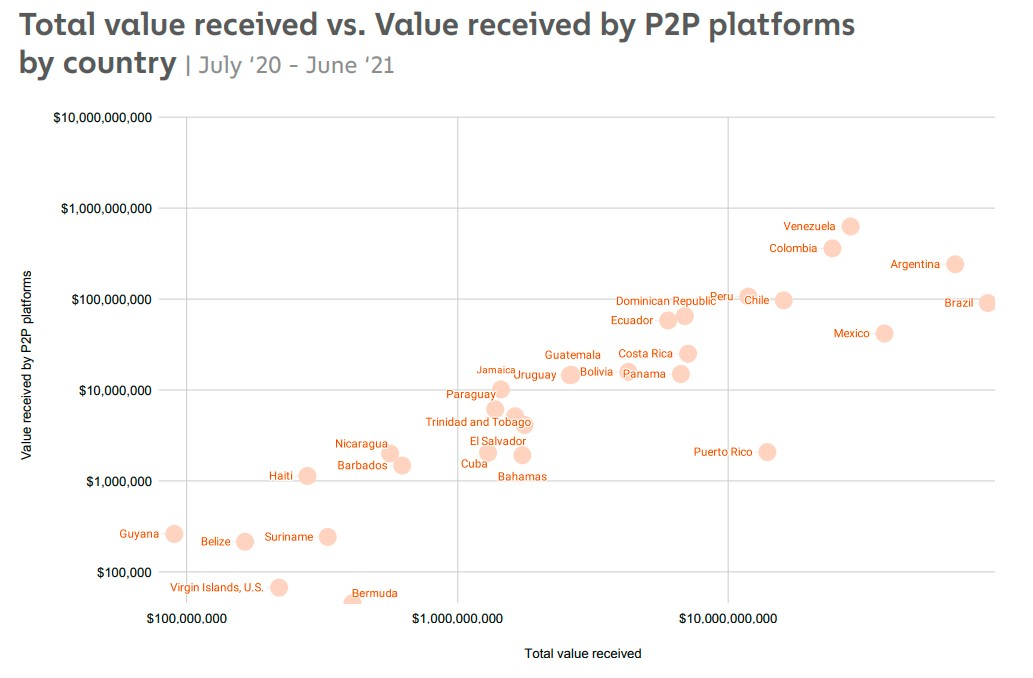
\includegraphics[width=1\textwidth]{images/C1/arg/arg_demanda (3).jpg}
        \vspace{-5mm}
        \caption*{Fuente: \href{https://blog.chainalysis.com/reports/2021-global-crypto-adoption-index/}{Chainalysis}}
        \end{figure}

\end{frame}